\documentclass[11pt]{article}
%\pagestyle{empty}
%\parindent0pt
%\usepackage{a4}
%\usepackage{amsmath,amssymb,bm,amsthm}
%\usepackage{amsfonts}
\usepackage{url,hyperref,multirow}
%\usepackage{float}
%\usepackage{color}
\usepackage{showlabels}
%\usepackage{mathtools}
%\usepackage{leftidx}
\usepackage{upgreek}
\usepackage{mathtools}
%\usepackage{amsmath}
\usepackage[all]{xy}\usepackage[latin1]{inputenc}        %accents
\usepackage[dvips]{graphics,graphicx}
\usepackage{amsfonts,amssymb,amsmath,color,mathrsfs, amstext}
\usepackage{amsbsy, amsopn, amscd, amsxtra, amsthm,authblk}
\usepackage{enumerate,algorithmicx,algorithm}
\usepackage{algpseudocode}
\usepackage{upref}
\usepackage{geometry}
%\geometry{left=3.5cm,right=3.5cm,top=3cm,bottom=3cm}
\usepackage[displaymath]{lineno}
%\linenumbers
\usepackage{float}
\usepackage{yhmath}
\usepackage{booktabs}
\usepackage{subcaption}
\usepackage{multirow}
\usepackage{makecell}
%\usepackage[colorlinks,
%            linkcolor=red,
%            anchorcolor=red,
%            citecolor=red
%            ]{hyperref}

\newtheorem{theorem}{Theorem}
\newtheorem{remark}{Remark}
\newtheorem{corollary}{Corollary}
\newtheorem{lemma}{Lemma}
\newtheorem{example}{Example}
\newtheorem{conjecture}{Conjecture}
\newtheorem{assumption}{Assumption}
\newtheorem{definition}{Definition}
\newtheorem{proposition}{Proposition}

\numberwithin{equation}{section} \numberwithin{theorem}{section}
\numberwithin{lemma}{section} \numberwithin{remark}{section}
\numberwithin{table}{section} \numberwithin{corollary}{section}
\numberwithin{example}{section} \numberwithin{conjecture}{section}
\numberwithin{assumption}{section}
\numberwithin{definition}{section}
\numberwithin{proposition}{section}
\newcommand{\zd}{\,\mathrm{d}}

\newcommand{\rd}[1]{{\color{red}#1}}
\newcommand{\bl}[1]{{\color{blue}#1}}
\newcommand{\ma}[1]{{\color{magenta}#1}}
\renewcommand{\o}{\emptyset}

\def\eps{\varepsilon}{\tiny {\normalsize }}
\parskip 0.1cm
 \setlength{\textwidth}{16cm}
 \setlength{\oddsidemargin}{0cm}
 \setlength{\textheight}{23cm}
 \setlength{\topmargin}{-1.5cm}


 \begin{document}

\title{The Brouwer degree in topology, geometry and analysis}

\author[1]{Mengyi Chen\thanks{E-mail: chenmengyi19@mails.ucas.ac.cn}}

\affil[1]{School of Mathematical Sciences, University of Chinese Academy of Sciences, Beijing 100049, China}
\maketitle
\begin{abstract}



​    We consider the definition of Brouwer degree for smooth mapping and some of its properties such as being locally constant and homotopy invariant. The main aim of this paper is to prove that winding number is a special case of Brouwer degree. To better prove this theorem, we generalize the definition of Brouwer degree and apply to the proof of the theorem. The geometric intuition of winding number are presented. 
​    We also present the applications of the Brouwer degree and the winding number in differential geometry.
\end{abstract}

\emph{Keywords:}
Brouwer degree; winding number; rotation index; differential topology; differential geometry.


\section{Introduction}
During this fall semester, I took some math courses including complex analysis, differential geometry, differential topology. When learning complex analysis, a course with the name 'analysis', seemed to be full of geometry intuition for me. The expression of the winding number:
\begin{equation}
    n(\gamma,p)=\frac{1}{2\pi i} \int_{\gamma}\frac{dz}{z-p},
\end{equation}
was of great magic beyond description. How could such a complex expression be an integer and depicted how many times the curve $\gamma$ curves around the point $p$. Then I came across the definition of rotation index in differential geometry, this time the expression was more friendly;
\begin{equation}
    \ the\  rotation \ index\  of\  \gamma = \frac{\theta(b)-\theta(a)}{2\pi},
\end{equation}
it seemed intuitive, but shortly after I confused the rotaiton index with the winding number since the former did not depend on a specific point while the latter does. It finally dawned on me that the rotation index was a special case of the winding number. The rotation index $\gamma =$ the winding number of $\gamma^{'}$ around 0.
Now I seemed to be relieved from the above problem, but when I learned differential topology,in Milnor's Topology from the differential point of view, there was a figure as follows:
\begin{figure}[H]
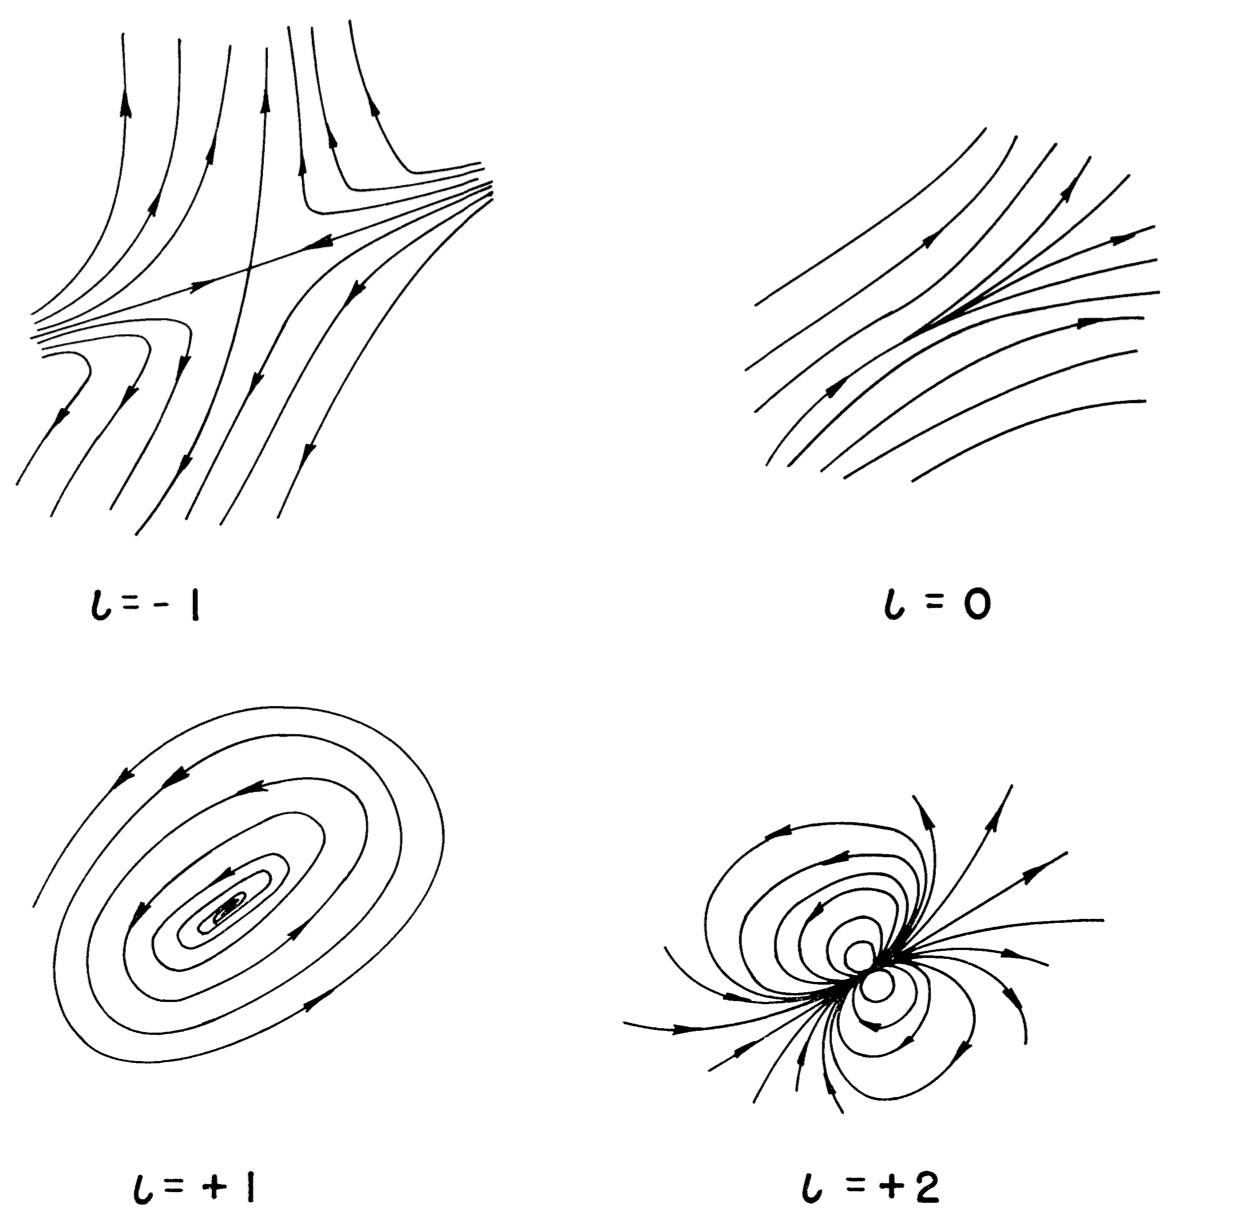
\includegraphics[width=11cm]{image/indexofvectorfields.png}
\centering
\caption{index of plane vector fields}
\end{figure}
There seemed to be an intuitive interpretation of the  index $ \iota$ of vector fields at the zero $z$ since the index $\iota$ could be computed  directly  through the figures,without knowing the specific expression of the vector fields. The index $\iota$ of a vector field $v$ is defined to be the Brouwer degree of  the map $\Bar{v}=\frac{v}{||v||}$. Then I tried to find out the connection between the winding number,the rotation index and the Brouwer degree,which occurred in complex analysis, differential geometry and differential topology respectively. I also tried to explore their geometric interpretation.

The outline of this paper is arranged as follows. In Section 2, we introduce the Brouwer degree and its generalization. The formulation of the fully proof that the winding number is a special case of Brouwer degree is presented in Section 3.We give some insight into differential geometry concerning the Brouwer degree in Section 4. Some conclusions and thoughts are given in Section 5.


\section{The Brouwer degree}
Let $M$ and $N$ be oriented n-dimensional manifolds without boundary. $M$ is compact and $N$ is connected. Let $f: M \rightarrow N$ be a smooth map. Then the Brouwer degree of $f$ is defined as follows:
\begin{definition}
Let $x\in M$ be a regular point of $f$, then $df_x: TM_x\rightarrow TN_{f(x)}$ is a linear isomorphism between oriented vector spaces.
Define
\begin{equation*}
    sign\  df_x:=\left\{\begin{array}{ll}
1 &\text{if}~df_x \  preserves\  orientation,
\\[0.1in]
-1 &\text{if}~df_x\  reverses\  orientation.
\end{array}\right. 
\end{equation*}
For any regular value $y \in N$ define 
\begin{equation}\label{try}
    deg(f;y)=\Sigma_{x\in f^{-1}(y)}\  sign\ df_x.
\end{equation}
In fact, the integer $deg(f;y)$ does not depend on the choice of regular value y\cite[$\S 5 \ Theorem A$]{milnor1997topology}. $\textbf{The degree of f}$ $:= deg(f;y),y$ is a regular value of $f$, and is  is usually denoted by $deg \ f$.
\end{definition}Note that since $M$ is compact and $f$ is continuous, $f^{-1}(y)$ is a closed subset of M and hence compact. According to the inverse function theorem, $f$ is a local diffeomorphism at any $x\in f^{-1}(y)$. Let $U_x$ be a neighborhood of $x\ $,$s.t. $ $f_{| U_x}$ is a diffeomorphism. 
$  \forall x, \overline{x} \in f^{-1}(y), x \neq \overline{x} $, $U_x \cap U_{\overline{x}}=\o$. $\cup_{x\in f^{-1}(y)} U_x$ is an open cover of $f^{-1}(y)$, hence there exists a finite subcover.
Then $f^{-1}(y)$ contains only finitely many points, so the sum in \ref{try} is a finite sum.

The Brouwer degree is a homotopy invariant, and we have the followint theorem:
\begin{theorem}\cite[$\S 5 \ Theorem B$]{milnor1997topology}
   If f is smoothly homotopic to g, then $deg\ f = deg \ g$.
\end{theorem}
Following we will generalize the definition of Brouwer degree as mentioned above. 
\begin{definition}\cite[$\S 1.2$]{cho2006topological}
Let $D \subset \mathbb{R}^n$ be open and bounded. $f:\Bar{D}\rightarrow \mathbb{R}^n$ is smooth. If $p \notin f(\partial D) \ and\  p\  is\  a \ regular \ value \ of\  f_{|D}$, then define 
\begin{equation}
    deg(f,D,p)=\Sigma_{x\in f^{-1}(p)} sign \ df_x,
\end{equation}
where $deg(f,D,p)=0$\ if $f^{-1}(p)=\o$.
\end{definition}
Note that $f^{-1}(p) \subset D \subset \Bar{D}, \Bar{D} \ is\  closed\  and\  bounded\  in\  \mathbb{R}^n,$ hence it is compact. Then $f^{-1}(p)$ is a finite set. In Definition 2.1 we require M to be compact, here we omit the requirement of compactness but $D $ is contained in the compact set $\Bar{D}$. In Definition 2.1, the codomain $N$ of $f$ is required to be connected. if $N$ is not connected, $N$ can be written as the union of its connected components, $N=\cup _{i\in J}N_i$. If $x,y$ belong to  the same connected component, and $x,y$ are regular values of $f$ , repeat the proof that the degree of $f$  is independent of the choice of regular value, we can see $deg(f;x)=deg(f;y)$. Hence we have the following Proposition:
\begin{proposition}
    Let $\Omega$ be a connected component of $ \mathbb{R}^n \setminus f(\partial D )$. $a,b$ are two regular values of $f_{|D}$ and $a,b \in \Omega$. Then 
    \begin{equation*}
        deg(f,D,a)=deg(f,D,b).
    \end{equation*}
$i.e.$,$deg(f,D,p)$ is a constant on any connected component of $ \mathbb{R}^n \setminus f(\partial D ),$
p is  a  regular  value  of $f_{|D}$.
\end{proposition}
Once the above proposition is established, we can define degree for \textbf{non-regular } values:
\begin{definition}
 Let $\Omega$ be a connected component of $ \mathbb{R}^n \setminus f(\partial D )$, and let $a\in \mathbb{R}^n\setminus f(\partial D )$,here a may not be a regular value. Choose $b\in \Omega$ and $b$ is a regular value  of $f_{|D}$. Then define:
 \begin{equation}
     deg(f,D,a)=deg(f,D,b),
 \end{equation}
 This is well-defined since the above definition does not depend on the choice of b. If  $b^{'} \in \Omega$ and  $b^'$ is another regular value  of $f_{|D}$, then $ deg(f,D,b)=deg(f,D,b^')$ by proposition 2.1. 
\end{definition}
Once the degree for non-regular values is established, we see that $deg(f,D,p)$ is a constant on any connected component of $\mathbb{R}^n\setminus f(\partial D )$.
Similar to theorem 2.2, we hava the following theorem:
\begin{theorem}\label{try1}\cite[\S 4 Prop 1.9]{outerelo2009mapping}
   Let $H:[0,1]\times \Bar{D} \rightarrow \mathbb{R}^n$ be a smooth mapping, and consider a point $a\in \mathbb{R}^n\setminus H([0,1]\times \partial D)$. Let $f=H(0,\cdotp)$, $g=H(1,\cdotp)$,then
   \begin{equation}
       deg(f,D,a)=deg(g,D,a)
   \end{equation}
\end{theorem}
Using Theorem \ref{try1}, we can prove the following important theorem:
\begin{theorem}[Boundary theorem]\cite[\S 4 prop 2.6]{outerelo2009mapping}Given two smooth mappings $f,g:\Bar{D}\rightarrow \mathbb{R}^n$ such that $f_{|\partial D}=g_{|\partial D}$ and given a point $a\notin f(\partial D)=g(\partial D)$, then
\begin{equation*}
    deg(f,D,a)=deg(g,D,a).
\end{equation*}
\begin{proof}
    Apply Theorem \ref{try1} to the homotopy  $H:[0,1]\times \Bar{D}\rightarrow \mathbb{R}^n,
    H(t,x)=(1-t)f(x)+tg(x)$. Note that 
    \begin{align*}
        H([0,1]\times \partial D)
        &=\cup_{t \in [0,1]} H_t(\partial D)\\
        &=\cup_{x\in \partial D,t \in [0,1]} (1-t)f(x)+tg(x)\\
    &= \cup_{x\in \partial D} \ g(x)\\
    &=f(\partial D)\\ &=g(\partial D),
 \end{align*}
 then $a\notin H([0,1]\times \partial D)=f(\partial D)$. Since $f=H(0,\cdotp),g=H(1,\cdotp),$ $deg(f,D,a)=deg(g,D,a)$.
\end{proof}
\end{theorem}
In fact, if we omit the assumption that $f$ is smooth, but only assume $f$ to be continuous, the Brouwer degree $deg(f,D,p)$ can also be defined\cite[\S 4.2]{outerelo2009mapping}.
Using \textbf{Witney approximation theorem for continuous maps}, one can find a smooth mapping $g$ which is homotopic to $f$. We can define $deg(f,D,p)=deg(g,D,p),\ p\notin f(\partial D)\cup g(\partial D)$, and this definition does not depend on the specific choice of $g$. Furthermore, $deg(f,D,a)$ shares all the properties that we have stated above when $f$ is smooth.
For detailed construction of degree of continuous mapping , one can refer to \cite[\S 4.2]{outerelo2009mapping}.


 In the next section, we introduce the winding number, and  prove that the winding number is a special case of the Brouwer degree.

\section{The winding number is a special case of Brouwer degree}
First we define the winding number of a curve $\gamma$ from the complex analysis point of view.
\begin{definition}
For a plane curve $\gamma :[a,b]\rightarrow \mathbb{C}$,  $\gamma $\ is continuous. $ \gamma$ is called \textbf{closed }if $\gamma(a)=\gamma(b)$.
\end{definition}
We can write $\gamma(t) = a(t) +\mathrm{i}b(t)$, and view $\gamma$ as a curve from $[a,b]$ to $\mathbb{R}^2$, $\gamma:[a,b]\rightarrow \mathbb{R}^2,t \mapsto (a(t),b(t))$, $\gamma$ is a continuous curve in $\mathbb{R}^2$.  
\begin{definition}
$\gamma$ is called \textbf{differentiable} if the derivative $a^{'} (t)$ and  $b^{'} (t)$  exist for $\forall t \in (a,b)$, and the left derivative exists for $a$, the right derivative exists for $b$.(Here differentiable does not mean smooth)
\end{definition}

The winding number is defined as follows:
\begin{definition}
Let $\gamma$ be a differentiable closed placne curve, $\gamma:[a,b]\rightarrow \mathbb{C}$, $a\in\mathbb{C}$ and $\gamma$ does not pass through the point a, then \textbf{the winding number of $\gamma$ with respect to p} is defined to be:
\begin{equation}
    n(\gamma,p)=\frac{1}{2\pi i} \int_{\gamma} \frac{dz}{z-p}.
\end{equation}
\end{definition}
From the knowledge of complex analysis, it is known that $n(\gamma,p)$ is an integar\cite[\S 4.2 Lemma 1]{complexanalysis1979ahlfors}. From the definition of $n(\gamma,p),$ $n(\gamma,p)$ is a continuous function of $z\neq p$. Then the winding number is locally constant since it is an integar. Now Let us see the winding number from an more intuitive point of view. 
Using the polar coordinate system, $\gamma(t)=p+r(t)e^{i\theta(t)}$($\theta(t)$is smooth),then 
\begin{align*}
  n(\gamma,p)
  &= \int_{\gamma} \frac{dz}{z-p} \\
  &=  \frac{1}{2\pi \mathrm{i}}\int_a^b \frac{d(p+r(t)\mathrm{e}^{\mathrm{i}\theta(t)})}{p+r(t)\mathrm{e}^{\mathrm{i}\theta(t)}-p} \\
  &=  \frac{1}{2\pi \mathrm{i}}\int_a^b \frac{\mathrm{e}^{\mathrm{i}\theta}dr+ir\mathrm{e}^{\mathrm{i}\theta}d\theta}{r\mathrm{e}^{\mathrm{i}\theta}}\\
  &=\frac{1}{2\pi \mathrm{i}}\int_a^b d(ln \ r) +\frac{1}{2\pi \mathrm{i}}\int_a^b \mathrm{i} d\theta\\
%  &=\frac{\theta(b)-\theta(a)}{2\pi}\\
  &=\frac{\theta(b)-\theta(a)}{2\pi}.
\end{align*}
It is intuitively seen that $n(\gamma,a)$ is an integar which represents how many times the curve $\gamma$ travels counterclockwise around the point $p$.

\begin{figure}[H]
\begin{subfigure}{0.5\textwidth}
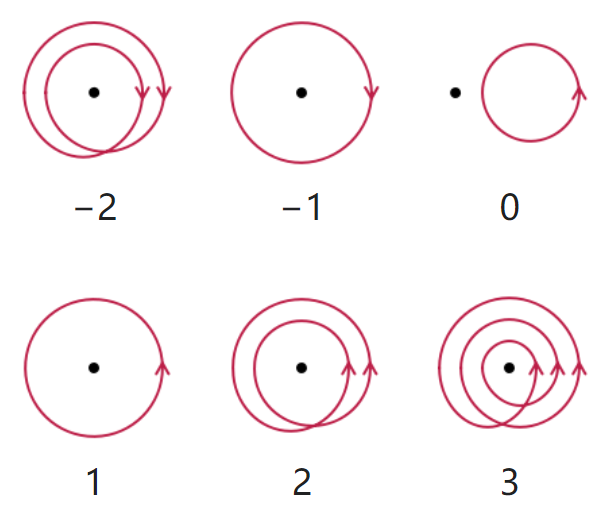
\includegraphics[width=0.9\linewidth, height=6cm]{image/windingnumber2.png} 
\caption{}
\end{subfigure}
\begin{subfigure}{0.5\textwidth}
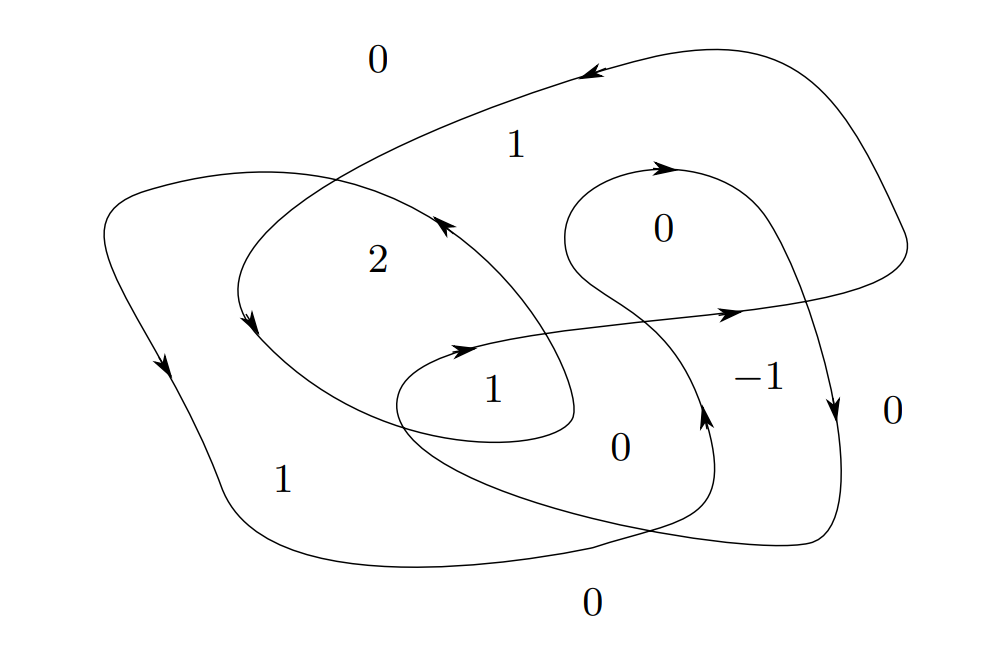
\includegraphics[width=0.9\linewidth, height=6cm]{image/windingnumber1.png}
\caption{}
\end{subfigure}
\caption{intuitive interpretation of winding number}
\end{figure}
Next, we want to prove that the winding number is in fact a special case of the Brouwer degree, which gives the winding number all the properties that the Brouwer degree has such as being locally constant and homotopy invariant.
First, we want to prove the following theorem:
\begin{theorem}
Let $\gamma$ be a differentiable closed plane curve, $\gamma:[a,b]\rightarrow \mathbb{C}$, then there exists a  differentiable surjective mapping from $S^1$ to $\gamma([a,b])$.For simplisity, we denote $\gamma([a,b])$ by $Im(\gamma)$.

To prove the theorem, we need the following lemma :

\begin{lemma}\cite[Theorem 22.2]{munkrestopology}
Let $p:X\rightarrow Y$ be a quotient map. Let $Z$ be a space and let $g:X\rightarrow Z$ be a map such that is consant on each set $p^{-1}({y})$, for $y\in Y$. Then g induces a map $f:Y\rightarrow Z$ such that $f \circ p =g$. This induced map $f$  is continuous if and only if $g$ is continuous; f is a quotient map if and only if g is a quotient map.
\end{lemma}
\[ 
\xymatrix@C=1.4cm@R=1.2cm{X\ar[rd]^{g}\ar[d]_{p}& \quad \\Y\ar@{.>}[r]_{f} & Z
}\]

\begin{proof}[proof of Theorem 3.1]
    Without loss of generality, we may assume $[a,b]=[0,2\pi]$ (if not, reparametrize $\gamma$).Let $\Bar{\gamma}:[0,2\pi]\rightarrow S^1,t\mapsto (\cos t,\sin t).$ $\Bar{\gamma}$ is surjective and continuous. If $C$ is a closed subset of $[0,2\pi]$, then $C$ is compact since  $[0,2\pi]$ is compact. $\Bar{\gamma}(C)$ is compact since $\Bar{\gamma}$ is continuous. Hence $\Bar{\gamma}(C)$ is closed since $S^1$ is hausdorff. We have now that $\Bar{\gamma}$ is also a closed map, then $\Bar{\gamma}$ is a quotient map.

    Let$\ \thicksim \ $be a equivalance relationship $s.t.\  0 \thicksim 2\pi$ and $\forall x\in $ $ (0,2 \pi),\ x$ is only element that is  equivalent to itself. Give $[0,2\pi]/\thicksim $ the quotient topology and let  $\pi:[0,2\pi]\rightarrow [0,2\pi]/\thicksim $ be the quotient map. Then there exists continuous maps $f \ and\  \Bar{f}$ $s.t. \ \Bar{f} \circ \pi =\Bar{\gamma} \ and \ f \circ \pi =\gamma$. Furthermore, $\Bar{f}$ is a quotient map since $\Bar{\gamma}$ is a quotient map. It is easy to see that $f$ is bijective from the definition, then $f^{-1}$ is continuous. 
    Finally we have the map $f\circ \Bar{f}^{-1}:S^1\rightarrow Im(\gamma) $, which is continuous and surjective. 
    
    Apply Lemma 3.1 to $\gamma^{'} and\  \Bar{\gamma}^'$.\ $ \Bar{\gamma}^{'}(t)=(-sint,cos t),$ which is continuous. Hence we have maps $g \ and \ \Bar{g}$  $s.t. \ \Bar{g} \circ \pi =\Bar{\gamma}^{'} \ and \ g \circ \pi =\gamma^{'}$. $\Bar{g}$ is bijectivem, then 
    $g\circ \Bar{g}^{-1}:S^1\rightarrow Im(\gamma) $ is well-defined. It is easy to see that $ g=f^{'},\Bar{g}=\Bar{f}^{'},$ then $g\circ \Bar{g}^{-1}=(f\circ \Bar{f}^{-1})^{'}$,which completes the proof of Theorem 3.1.
\end{proof}
\[ \xymatrix@C=3cm@R=2cm{\quad&\left[0,2\uppi \right]/\sim\ar[ld]_{\bar{f}}\ar[rd]^{f}&\quad\\S^1&\left[0,2\uppi \right]\ar[l]_{\bar{\gamma}}\ar[u]_{\uppi}\ar[r]^{\gamma}&Im\gamma\subset\mathbb{C}
} \]
\[ \xymatrix@C=3cm@R=2cm{\quad&\left[0,2\uppi \right]/\sim\ar[ld]_{\bar{g}}\ar[rd]^{g}&\quad\\S^1&\left[0,2\uppi \right]\ar[l]_{\bar{\gamma}^{'}}\ar[u]_{\uppi}\ar[r]^{\gamma^{'}}&Im\gamma\subset\mathbb{C}
} \]
\end{theorem}
For any differentialble closed plane curve $\gamma:[a,b]\rightarrow \mathbb{C}$, we can view $\gamma $ as a differentiable  surjective from $S^1$ to  $Im(\gamma)$. Using the polar coordinate systems, $\gamma: S^1\rightarrow \mathbb{C},\theta \mapsto \gamma(\theta)$. Suppose $\Tilde{\gamma}:\overline{B(0,1)} \rightarrow \mathbb{C}$ is a differentiable extension of  $\gamma$(such a extension exists because if we set $\Tilde{\gamma}(r,\theta)=r\gamma(\theta)$, then $\Tilde{\gamma}$ satisfies the requirement), we have the following theorem:
\begin{theorem}
Assume $p\notin Im(\gamma)$,Then 
\begin{equation}
    n(\gamma,p)=\frac{1}{2\pi i}\int_{\gamma}\frac{dz}{z-p} =deg(\Bar{\gamma},B(0,1),p),
\end{equation}
$n(\gamma,p)$ does not depend on the choice of the extension $\Bar{\gamma}$.
\end{theorem}
\begin{proof}
    By sard's lemma, the critical value of $\Bar{\gamma}$ is dense in $\mathbb{C}$. We have stated before that the winding number is locally constant, and the Brouwer degree $deg(f,D,a)$ for a non-regular value $a$ are  defined to be $deg(f,D,b)$, where $ b $ and $ a  $ are in the same connected component. Then we only need to prove the theoerem when $p$ is a regular value.
    
    Let $\Bar{\gamma}^{-1}(p)={\{z_1,\cdots ,z_k\}}$. $d\Bar{\gamma}_{z_i}\neq 0,i=1, \cdots ,k$. Then by inverse function theorem,there exists $V_i=B(z_i,\epsilon)$ $s.t.\  \Bar{\gamma}_{|V_i} $is a homeomorphism and $sign\  d\Bar{\gamma}_{z_i}=sign\  d\Bar{\gamma}_{z},\forall z\in V_i$. Take $\epsilon$ small enough such that $\Bar{V_i}$ are mutually disjoint. Let $S_i= \partial V_i,$ then $\Bar{\gamma}(S_i)$ is a differentiable closed curve $s.t.\  a$ lies in its interior. $\Bar{\gamma}(S_i)$   winds exactly once around $a$, $\Bar{\gamma}(S_i)$ has the same orientation as $S_i$ if $sign \ d\Bar{\gamma}_{z_i}>0$ and the opposite if $sign \ d\Bar{\gamma}_{z_i}<0$.   Then 
    \begin{equation}
        \int_{\Bar{\gamma}(S_i)} \frac{dz}{z-p}= sign \ d\Bar{\gamma}_{z_i}.
    \end{equation}
    Now set $U=\overline{B(0,1)} \cup_{i=1}^k V_i$. Then $|\Bar{\gamma}(z)-p|>\alpha$ in $U$ for some $\alpha>0 $. Divide $U$ into small subsets $R_j$, $s.t. |\Bar{\gamma}(z)-\Bar{\gamma}(w)|<\alpha,\forall z,w \in R_j$ on each $R_j$.
    Choose $z\in \partial R_j$, then $|\Bar{\gamma}(z)-p|>\alpha$. $\forall w\in \partial R_j$,$ |\Bar{\gamma}(z)-\Bar{\gamma}(w)|<\alpha$, then $\Bar{\gamma}(\partial R_j)$ does not wind around $a$, hence
    \begin{equation}
         \int_{\Bar{\gamma}(\partial R_j)} \frac{dz}{z-p}=0
    \end{equation}
    Then
\begin{align*}
    n(\gamma,p)&=\frac{1}{2\pi i} \int_{\gamma} \frac{dz}{z-p} \\
    &=\frac{1}{2\pi i} \int_{\partial\overline{B(0,1)}} \frac{dz}{z-p}\\
     &=\frac{1}{2\pi i} \int_{\partial ( \cup_j R_j \cup_{i=1}^k V_i )} \frac{dz}{z-p}\\
     &= \cup_j \frac{1}{2\pi i} \int_{\partial R_j} \frac{dz}{z-p} +\cup_{i=1}^k \frac{1}{2\pi i} \int_{\partial V_i} \frac{dz}{z-p} \\
     &= 0+ \sum_{i=1}^k sign\ d\bar{\gamma}_{z_i}\\
     &=deg(\bar{\gamma},B(0,1),p).
\end{align*}
Suppose $\Bar{\gamma}$ and $\Tilde{\gamma}$ are two differentiable extention of $\gamma$. We have $\Bar{\gamma}_{|S^1}=\Tilde{\gamma}_{|S^1}$. Then by the boundary Theorem $deg(\Bar{\gamma},B(0,1),p)=deg(\Tilde{\gamma},B(0,1),p)$, which completes the proof.
\end{proof}
From Theorem 3.2 we know that $n(\gamma,p)$ have the following propoties:

$\mathbb{\mathit{1}})$: If $z\ and  \ w$ belong to the same connected component of $\mathbb{C} \setminus \gamma$, then $n(\gamma,z)=n(\gamma,w)$.

$\mathbb{\mathit{2}})$:Let $\gamma $ and $\zeta$ are two homotopic curve that do not pass $p$. Suppose $H:[0,1]\times \overline{B(0,1)} \rightarrow \mathbb{C}$  is a homotopy between $\gamma$ and $\zeta$ and $p \notin H([0,1]\times S^1)$.
Then $n(\gamma,p)=n(\zeta,p)$. 

\section{Brouwer degree in differential geometry}
In differential geometry, we only consider curves that are smooth. For a smooth plane curve $\gamma:[a,b]\rightarrow \mathbb{R}^2$, we can always reparametrize it,$s.t.\  \gamma$ is of unit speed.
\begin{definition}
Let $\gamma: [a,b]\rightarrow \mathbb{R}^2 $ be a plane curve. It is called \textbf{regular} if its speed $|\gamma^{'}(t)| \neq 0,\forall t\in [a,b]$. It is called \textbf{closed} if 
\begin{equation}
    \gamma(a)=\gamma(b),\gamma^{'}(a)=\gamma^{'}(b),\gamma^{''}(a)=\gamma^{''}(b),\cdots
    \end{equation}
\end{definition}
In differential geometry, we have the following theorem:
\begin{theorem}\cite[Prop 1.39]{tapp2016differential}
If $\gamma:[a,b]\rightarrow  \mathbb{R}^2$ is a unit-speed plane curve, then there exists a smooth angle function, $\theta:[a,b]\rightarrow \mathbb{R}$,$s.t.$ \forall $t \in [a,b]$,we have:
\begin{equation}
    \mathbf{v}(t)=(cos\theta(t),sin\theta(t)),
\end{equation}
where $\theta (t)=\int_{t_0}^t \kappa _s(u)du+\theta_0$,$\kappa_s$ is the signed curvature of $\gamma$.

\end{theorem}
Then we have the definition of the rotation index:
\begin{definition}
Let $\gamma:[a,b]\rightarrow \mathbb{R}^2$ be a unit-speed clsoed plane curve. The \textbf{rotation index} of $\gamma$ is defined to be 
\begin{equation}
    \frac{1}{2\pi}(\theta(b)-\theta(a)),
\end{equation}
where $\theta$ is the angle function.To simplify notation, write $ind \ \gamma$ to denote the rotation index of $\gamma$.
\end{definition}
We have that 
\begin{equation}
\gamma^{'}(t)=\mathbf{v}(t)=(\cos \ \theta(t),\sin\ \theta(t)),
\end{equation}
$\gamma^{'}(t)$ lies on $S^1$ since $\gamma$ is of unit-spped.
Next we will prove that $ind \ \gamma$ is in fact $n(\gamma^{'},0)$.
\begin{theorem}
ind  $\gamma$ = $n(\gamma^{'},0)$.Then the rotation index of $\gamma$ is an integar.
\end{theorem}
\begin{proof}
    Identify $\mathbb{R}^2$ with $\mathbb{C}$.Choose polar coordinate,then $\gamma^{'}:[a,b]\rightarrow \mathbb{C},t\mapsto e^{i\theta(t)}$.
    \begin{align*}
        n(\gamma^{'},0)&=\frac{1}{2\pi \mathrm{i}}\int_{\gamma}\frac{dz}{z}\\
        &=\frac{1}{2\pi \mathrm{i}}\int_{a}^b\frac{d\mathrm{e}^{\mathrm{i}\theta(t)}}{\mathrm{e}^{\mathrm{i}\theta(t)}}\\
        &=\frac{1}{2\pi \mathrm{i}}\int_{a}^b id\theta\\
        &=\frac{\theta(b)-\theta(a)}{2\pi}.
    \end{align*}
\end{proof} 
Theorem 4.2 yields geometry intuitition for $ind\  \gamma$. The rotation index is an integar that depicts how many times the tangent speed vector winds around.Note that the rotaion index is irrelavent to the choice of a point $p \in \mathbb{C}$.
\begin{figure}[H]
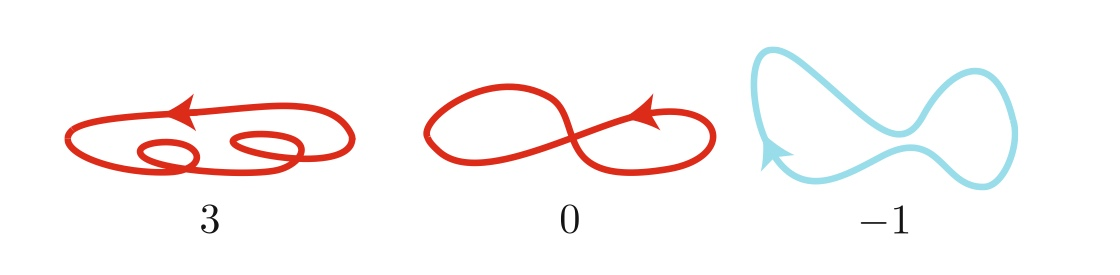
\includegraphics[width=11cm]{image/rotation index.PNG}
\centering
\caption{the rotation indices of some closed plane curves}
\end{figure}
Let $\mathbf{n}$ be the normal vector along $\gamma$ that gives the orientation of $\gamma$. Then the rotaiton index of $\gamma$ can also be viewed as the winding number of $\mathbf{n}$ around 0.

A deep theorem(\textbf{Hopf's Umlaufsatz}) in differential geometry states that the rotation index of a simply closed plane curve $\gamma$ is either 1 or -1 with respect to whether $\gamma$ is positively oriented or negatively oriented. 
\section{Conclusion and thoughts}

In this paper, we have presented the connection between the Brouwer degree, the winding number and the rotation index. The deep connection gives me full insight to the profound relationship between analysis and geometry.

When I wrote this paper, the biggest difficulty that I came across lied on the different restrictions of the mapping. In milnor's book, the Brouwer degree is defined for smooth maps. At first I wanted to use this definition and proved that the winding number is a special case of the Brouwer degree.
However, in complex analysis, we consider differential closed curve, which may not be smooth(Although holomorphic function is infinitrly differentiable, closed curve in $C$ are only defined in a real interval, thus not holomorphic).
Initially I decided to prove the theorem only for smooth closed curve $\gamma$, but in the proof, the extension of $\gamma$ is used. $Tietze\  extension \ theorem$ only tells us how to extend a continuous function, but how can I extend a smooth function(In fact, in this problem this is possible, I only need to define $\Bar{\gamma}(r,\theta)=r\gamma(\theta)$, however I did not find this at the very beginning)? 

Then I generalized the definition of Brouwer degree, but without proof, so that it is suitable for continuous function. The winding number is defined for differentiabl closed map. It disappointed me that the Tietze extension theorem still doed not apply. Just at the very time when my building of the paper was going to collapse, I found a differentiable extension for the differential map $\gamma:S^1\rightarrow \mathbb{C},\theta\mapsto \gamma(\theta)$, namely $\Bar{\gamma(r,\theta)=r\gamma(\theta)}$. With this differentiable extension I finished this paper. 
The above extension is smooth if $\gamma$ is smooth. 

So if I restricted the discussion of $\gamma$ only for smooth curves $\gamma$, this paper could be more concise, but may not as general. And since I have finished the proof for only differentiable curve, I do not have the heart to delete them. 

From preparing the latex lecture notes, delivering a speech ,communicating with teammates, to wrting this paper, I have benifited a lot from one semester's Seminar on Geometry.  The set of the course syllabus is rather reasonalble, it is challenging but not extremly difficult to frustrate us. Thanks for the professor and the teaching assistant's devotion to this seminar. And thanks my own endeavor that enable me to experience the fabulous geometry.

\bibliographystyle{plain}
\bibliography{DifferentialTopology}
 \end{document}
